%input macros (i.e. write your own macros file called MacroFile1.tex)
%\newcommand{\PdfPsText}[2]{
  \ifpdf
     #1
  \else
     #2
  \fi
}

\newcommand{\IncludeGraphicsH}[3]{
  \PdfPsText{\includegraphics[height=#2]{#1}}{\includegraphics[bb = #3, height=#2]{#1}}
}

\newcommand{\IncludeGraphicsW}[3]{
  \PdfPsText{\includegraphics[width=#2]{#1}}{\includegraphics[bb = #3, width=#2]{#1}}
}

\newcommand{\InsertFig}[3]{
  \begin{figure}[!htbp]
    \begin{center}
      \leavevmode
      #1
      \caption{#2}
      \label{#3}
    \end{center}
  \end{figure}
}


%%% Local Variables: 
%%% mode: latex
%%% TeX-master: "~/Documents/LaTeX/CUEDThesisPSnPDF/thesis"
%%% End: 


\documentclass[oneside,12pt]{article}


% turn of those nasty overfull and underfull hboxes
\hbadness=10000
\hfuzz=50pt

% Put all the style files you want in the directory StyleFiles and usepackage like this:
%\usepackage{StyleFiles/watermark}
\usepackage{url}
\usepackage{nomencl}
\usepackage{makeidx}
\usepackage{graphicx}
\usepackage{pgfplots}
\usepackage{longtable}
\usepackage{amssymb, amsmath}
\usepackage{algorithm}
\usepackage{algpseudocode}
\usepackage{multirow}
\usepackage{rotating}
\usepackage{float}
%% The amsthm package provides extended theorem environments
%% \usepackage{amsthm}
\usepackage{booktabs}
\usepackage{tikz}


\usetikzlibrary{patterns}
\usetikzlibrary{arrows,positioning,fit}

%\usepackage{glossary}
%\makenomenclature
%\makeindex
%\makeglossary
%\usepackage{natbib}

\newcommand{\uvec}{\mathbf{u}}
\newcommand{\vvec}{\mathbf{v}}
\newcommand{\tab}{\hspace*{2em}}

\begin{document}

\renewcommand\baselinestretch{1.2}
\baselineskip=18pt plus1pt

\pgfplotsset{
every axis/.append style={
        legend pos=south east,
        scaled ticks=false,
        xlabel=Total cost (ZAR),
        ylabel=Service level,
        xtick={400000,600000,800000,1000000,1200000}
        }
        }


\begin{figure}
\label{fig:CostScenarios}
\centering
    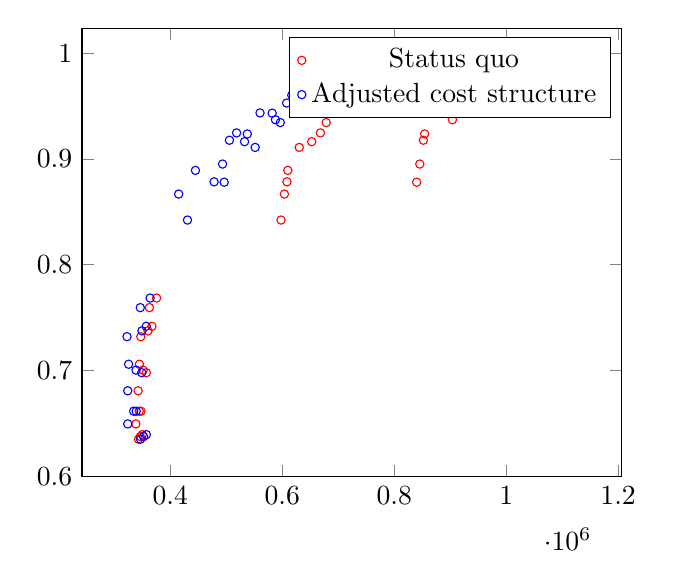
\begin{tikzpicture}
        \begin{axis}[
        %legend cell align=left,
        %legend pos=south east,
        %scaled ticks=false,
        %xlabel=Total cost (ZAR),
        %ylabel=Service level,
        %xtick={400000,600000,800000,1000000,1200000}
        ]
        \addplot[
        color=red,only marks, mark options={
        fill=white,
        scale=0.75},
        mark=o
        ]
        coordinates{
(344900,0.7058)
(360190,0.73737)
(367250,0.74169)
(347290,0.73187)
(362750,0.75933)
(375510,0.7684)
(609960,0.88915)
(686960,0.94346)
(794190,0.96191)
(603850,0.86673)
(668190,0.92459)
(762760,0.95519)
(852110,0.91763)
(939310,0.96023)
(1020100,0.98046)
(845710,0.89513)
(920940,0.94323)
(1052100,0.97741)
(338540,0.64934)
(344500,0.66141)
(347670,0.66136)
(342550,0.68068)
(351330,0.70025)
(357260,0.69781)
(608380,0.87831)
(678570,0.93434)
(747620,0.94962)
(597800,0.84216)
(652640,0.91626)
(736140,0.94812)
(854340,0.92357)
(941970,0.96501)
(1064100,0.98118)
(840110,0.87795)
(903940,0.93706)
(1017400,0.97236)
(343250,0.63491)
(346570,0.63739)
(350070,0.63922)
(630350,0.91086)
(713440,0.94987)
(767430,0.94747)
(874290,0.95281)
(979310,0.97505)
(1126000,0.98824)
        };
        \addplot[
        color=blue,only marks, mark options={
        fill=white,
        scale=0.75},
        mark=o
        ]
        coordinates{
        (325600,0.7058)
(349410,0.73737)
(357050,0.74169)
(322730,0.73187)
(346450,0.75933)
(364020,0.7684)
(444980,0.88915)
(560300,0.94346)
(710760,0.96191)
(415010,0.86673)
(518450,0.92459)
(664060,0.95519)
(505630,0.91763)
(617000,0.96023)
(817240,0.98046)
(493400,0.89513)
(582050,0.94323)
(771020,0.97741)
(324070,0.64934)
(334550,0.66141)
(339160,0.66136)
(324050,0.68068)
(338790,0.70025)
(349010,0.69781)
(478300,0.87831)
(596500,0.93434)
(699130,0.94962)
(430720,0.84216)
(532700,0.91626)
(664210,0.94812)
(537590,0.92357)
(675420,0.96501)
(874940,0.98118)
(496270,0.87795)
(587850,0.93706)
(770980,0.97236)
(346780,0.63491)
(352390,0.63739)
(357310,0.63922)
(551660,0.91086)
(680600,0.94987)
(754600,0.94747)
(607800,0.95281)
(783850,0.97505)
(1018500,0.98824)
        };
            \legend{Status quo, Adjusted cost structure}
        \end{axis}
    \end{tikzpicture}
%\caption{Overall difference between status quo and adjusted cost structures}
\end{figure}

\end{document}
